% =====================================================================
%  CIS 111 -- Week 11: CLI (Command Line Interface)
%  LaTeX Beamer conversion of cis111-w11-CLI-20251208.pptx
%
%  Compile with:  pdflatex cis111-w11-CLI.tex   (run twice)
% =====================================================================
\documentclass[aspectratio=43,10pt,t]{beamer}

\usepackage[utf8]{inputenc}
\usepackage[T1]{fontenc}
\usepackage[scaled=0.92]{helvet}   % Arial-like sans (as in the original)
\usepackage{courier}               % Courier (as in the original code)
\renewcommand{\familydefault}{\sfdefault}
\usepackage{graphicx}
\usepackage{listings}
\usepackage{xcolor}
\usepackage{tikz}
\usetikzlibrary{arrows.meta}
% crossed-out value in the trace table (like the hand-drawn original)
\newcommand{\sout}[1]{\tikz[baseline=(t.base)]{\node[inner sep=1pt](t){#1};\draw[thin] (t.south west)--(t.north east);}}

% ---------------------------------------------------------------------
%  Hidden slides
%  The Self Check slides were *hidden* in the original PowerPoint.
%  They are kept here but hidden by default.
%    \newcommand{\hiddenslides}{0}   -> hide them (like the original)
%    \newcommand{\hiddenslides}{1-}  -> show them
% ---------------------------------------------------------------------
\newcommand{\hiddenslides}{0}

% ---------------------------------------------------------------------
%  Colours
% ---------------------------------------------------------------------
\definecolor{titlerule}{HTML}{FFD966}   % yellow rule under frame titles
\definecolor{callout}{HTML}{FFE14D}     % yellow call-out boxes
\definecolor{codebg}{HTML}{DDDDDD}      % grey code background
\definecolor{syntaxteal}{HTML}{1F8C8C}  % "Syntax 6.x" headings
\definecolor{kwblue}{HTML}{1F3FA8}
\definecolor{cmtteal}{HTML}{2A8FBF}
\definecolor{strred}{HTML}{B22222}

% ---------------------------------------------------------------------
%  Beamer look
% ---------------------------------------------------------------------
\setbeamertemplate{navigation symbols}{}
\setbeamercolor{normal text}{fg=black}
\setbeamercolor{structure}{fg=black}
\setbeamercolor{frametitle}{fg=black}
\setbeamerfont{frametitle}{series=\bfseries,size=\large}
\setbeamertemplate{frametitle}{%
  \vskip2mm
  \usebeamerfont{frametitle}\insertframetitle\par
  \vskip-0.5mm
  {\color{titlerule}\rule{0.76\paperwidth}{1.3pt}}\par
}
\setbeamertemplate{itemize item}{\small$\blacksquare$}
\setbeamertemplate{itemize subitem}{\scriptsize$\blacksquare$}
\setbeamertemplate{itemize subsubitem}{\tiny$\blacksquare$}
\setbeamerfont{itemize/enumerate body}{size=\small}
\setbeamerfont{itemize/enumerate subbody}{size=\small}
\setbeamerfont{itemize/enumerate subsubbody}{size=\small}
\setbeamertemplate{footline}{%
  \hfill\color{gray}\scriptsize\insertframenumber\hspace*{4mm}\vspace*{2mm}}
\setbeamersize{text margin left=7mm,text margin right=7mm}

% ---------------------------------------------------------------------
%  Code listings (Java)
% ---------------------------------------------------------------------
\lstdefinestyle{java}{
  language=Java,
  basicstyle=\ttfamily\scriptsize,
  keywordstyle=\color{kwblue},
  commentstyle=\color{cmtteal},
  stringstyle=\color{strred},
  backgroundcolor=\color{codebg},
  frame=single, rulecolor=\color{codebg}, framesep=3pt,
  columns=fullflexible, keepspaces=true,
  showstringspaces=false, tabsize=4,
  xleftmargin=3pt, xrightmargin=3pt,
  aboveskip=4pt, belowskip=4pt,
  upquote=true,
}
\lstset{style=java}
% plain console output (yellow box)
\lstdefinestyle{output}{
  language={}, basicstyle=\ttfamily\scriptsize\color{strred},
  backgroundcolor=\color{callout}, rulecolor=\color{callout},
  commentstyle={}, keywordstyle={}, stringstyle={},
}

% full program listings (with line numbers, as in the textbook)
\definecolor{progbg}{HTML}{EDEDED}
\definecolor{lineno}{HTML}{1F5FAF}
\lstdefinestyle{program}{
  style=java,
  basicstyle=\ttfamily\fontsize{6.2}{7.2}\selectfont,
  backgroundcolor=\color{progbg}, rulecolor=\color{progbg},
  numbers=left, numberstyle=\ttfamily\bfseries\fontsize{6}{7.2}\selectfont\color{lineno},
  numbersep=6pt, xleftmargin=14pt, framexleftmargin=0pt,
  breaklines=true, breakindent=24pt, breakatwhitespace=true,
}
% "Program Run" box:  \programrun{width}{content}
\newcommand{\programrun}[2]{%
  \begin{minipage}{#1}
    {\bfseries\small\color{lineno} Program Run}\par\vskip1mm
    {\setlength{\fboxsep}{4pt}\colorbox{progbg}{%
      \parbox{\dimexpr\linewidth-8pt\relax}{\ttfamily\fontsize{6}{7.4}\selectfont #2}}}
  \end{minipage}}
\newcommand{\userinput}[1]{\textcolor{lineno}{#1}}

% ---------------------------------------------------------------------
%  Helpers
% ---------------------------------------------------------------------
\newcommand{\code}[1]{\texttt{#1}}
% yellow call-out box:  \callout[width]{text}
\newcommand{\callout}[2][\linewidth]{%
  {\setlength{\fboxsep}{3pt}\colorbox{callout}{%
    \parbox{\dimexpr#1-6pt\relax}{\raggedright\footnotesize #2}}}}
% small yellow label (replaces the arrow labels "reference"/"value")
\newcommand{\ptag}[1]{{\setlength{\fboxsep}{1.5pt}\colorbox{callout}{\scriptsize #1}}}
\newcommand{\answer}{\textbf{Answer:}\ }
\newcommand{\syntaxtitle}[2]{\textcolor{syntaxteal}{Syntax #1}\ #2}

% ---------------------------------------------------------------------

\definecolor{dividerred}{HTML}{C00000}
\definecolor{cellbg}{HTML}{CFE8E6}
\definecolor{cellrule}{HTML}{8FC6C1}
% section divider slide (red centred title, as in the original)
\newcommand{\dividerslide}[1]{%
  \begin{frame}[plain,c]
    \centering{\Large\bfseries\color{dividerred}#1\par}
  \end{frame}}
% shell command in a grey box
\newcommand{\shell}[1]{{\setlength{\fboxsep}{3pt}\colorbox{codebg}{\ttfamily\footnotesize #1}}}

\title{CLI (Command Line Interface)}
\date{}

\begin{document}

% =====================================================================
%  1  Title
% =====================================================================
\begin{frame}{CLI (Command Line Interface)}
\end{frame}

% =====================================================================
%  2  Section: Command Line Interface
% =====================================================================
\section{Command Line Interface}
\dividerslide{Command Line Interface}

% =====================================================================
%  3  Chapter Goals
% =====================================================================
\begin{frame}{Chapter Goals}
  \vskip8mm
  \begin{itemize}
    \setlength{\itemsep}{4mm}
    \item What is CLI?
    \item Java \& CLI
    \item To process command line arguments
  \end{itemize}
\end{frame}

% =====================================================================
%  4  What is CLI?
% =====================================================================
\begin{frame}{What is CLI?}
  \vskip6mm
  \begin{itemize}
    \item A \textbf{Command Line Interface (CLI)} is a text-based way to interact with
          software, where users type commands instead of using a graphical interface (GUI).
  \end{itemize}
\end{frame}

% =====================================================================
%  5  Java & CLI
% =====================================================================
\begin{frame}{Java \& CLI}
  \begin{itemize}
    \item Java provides built-in classes to handle input/output:
      \begin{itemize}
        \setlength{\itemsep}{2mm}
        \item \code{System.in}\quad Reads input from the terminal
        \item \code{System.out}\quad Prints output to the console
        \item \code{Scanner}\quad Parses user input (numbers, strings, etc.)
        \item \code{args[]}\quad Accesses command-line arguments
      \end{itemize}
  \end{itemize}
\end{frame}

% =====================================================================
%  6  Command-Line Arguments (args[])
% =====================================================================
\begin{frame}[fragile]{Command-Line Arguments (\texttt{args[]})}
  \begin{itemize}
    \item How \textbf{\code{args[]}} Works:
      \begin{itemize}
        \item Pass arguments when running the program in Bash (or PowerShell etc):
      \end{itemize}
  \end{itemize}
\begin{lstlisting}[language={},linewidth=0.62\linewidth,xleftmargin=0.12\linewidth]
java MyApp.java arg1 arg2
\end{lstlisting}
  \hspace*{0.12\linewidth}{\small Here}
\begin{lstlisting}[linewidth=0.62\linewidth,xleftmargin=0.12\linewidth]
args[0] = "arg1",
args[1] = "arg2"
\end{lstlisting}
\end{frame}

% =====================================================================
%  7  Example: Calculator
% =====================================================================
\begin{frame}[fragile]{Example: Calculator}
\begin{lstlisting}[basicstyle=\ttfamily\fontsize{6.3}{7.4}\selectfont]
public class Calculator {
    public static void main(String[] args) {
        if (args.length != 3) {
            System.out.println("Usage: java Calculator <num1> <+|-|*|/> <num2>");
            return;
        }
        double num1 = Double.parseDouble(args[0]);
        double num2 = Double.parseDouble(args[2]);
        String op = args[1];

        switch (op) {
            case "+": System.out.println(num1 + num2); break;
            case "-": System.out.println(num1 - num2); break;
            case "*": System.out.println(num1 * num2); break;
            case "/": System.out.println(num1 / num2); break;
            default: System.out.println("Invalid operator!");
        }
    }
}
\end{lstlisting}
  \vskip2mm
\begin{lstlisting}[language={},basicstyle=\ttfamily\scriptsize\color{green!45!black}]
$ java Calculator.java 5 '*' 3
15.0
\end{lstlisting}
  {\scriptsize\color{gray} Quote the \code{*}; otherwise the shell expands it to the file names in the current directory.}
\end{frame}

% =====================================================================
%  8  Section: Command Line Arguments
% =====================================================================
\section{Command Line Arguments}
\dividerslide{Command Line Arguments}

% =====================================================================
%  9  Command Line Arguments
% =====================================================================
\begin{frame}{Command Line Arguments}
  \begin{itemize}
    \item Text based programs can be `parameterized' by using command line arguments
      \begin{itemize}
        \item Filename and options are often typed after the program name at a command prompt:
      \end{itemize}
  \end{itemize}
  \vskip1mm
  \begin{center}
    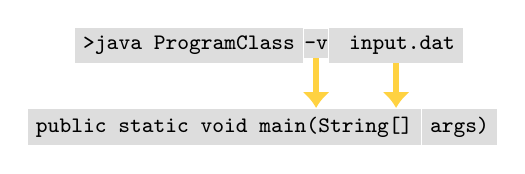
\begin{tikzpicture}[font=\ttfamily\footnotesize,
        part/.style={fill=codebg,inner xsep=0pt,inner ysep=3pt,anchor=base west}]
      \node[part,inner xsep=3pt] (c1) at (0,0) {>java ProgramClass\ };
      \node[part] (c2) at (c1.base east) {-v};
      \node[part,inner xsep=3pt] (c3) at (c2.base east) {\ input.dat};
      \node[part,inner xsep=3pt] (s1) at (-0.6,-1.05) {public static void main(String[]\ };
      \node[part,inner xsep=3pt] (s2) at (s1.base east) {args)};
      \foreach \n in {c2,c3}
        \draw[-{Latex[length=2mm,width=3.5mm]},line width=2.4pt,callout!85!orange]
          (\n.south) -- (\n.south |- s2.north);
    \end{tikzpicture}
  \end{center}
  \begin{itemize}
    \item[]
      \begin{itemize}
        \item Java provides access to them as an array of \code{String}s parameter to the
              \code{main} method named \code{args}
      \end{itemize}
  \end{itemize}
  \vskip1mm
  \hspace*{0.25\linewidth}{\setlength{\fboxsep}{4pt}\colorbox{callout!60}{%
    \ttfamily\footnotesize\begin{tabular}{@{}l@{}}args[0]: "-v"\\ args[1]: "input.dat"\end{tabular}}}
  \vskip2mm
  \begin{itemize}
    \item[]
      \begin{itemize}
        \item The \code{args.length} variable holds the number of \code{args}
        \item Options (switches) traditionally begin with a dash `\code{-}'
      \end{itemize}
  \end{itemize}
\end{frame}

% =====================================================================
%  10  Caesar Cipher Example
% =====================================================================
\begin{frame}{Caesar Cipher Example}
  \begin{itemize}
    \item Write a command line program that uses character replacement (Caesar cipher) to:
      \begin{itemize}
        \item Encrypt a file provided input and output file names\\[1mm]
              \shell{>java CaesarCipher input.txt encrypt.txt}
        \item Decrypt a file as an option\\[1mm]
              \shell{>java CaesarCipher -d encrypt.txt output.txt}
      \end{itemize}
  \end{itemize}
  \vskip5mm
  \centering
  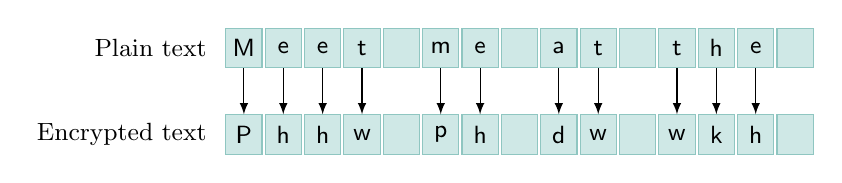
\begin{tikzpicture}[
      cell/.style={draw=cellrule,fill=cellbg,minimum width=4.6mm,minimum height=5mm,
                   inner sep=0pt,font=\sffamily\small},
      lbl/.style={font=\rmfamily\small,anchor=east}]
    \def\plain{{"M","e","e","t"," ","m","e"," ","a","t"," ","t","h","e"," "}}
    \def\enc{{"P","h","h","w"," ","p","h"," ","d","w"," ","w","k","h"," "}}
    \node[lbl] at (-0.25,0) {Plain text};
    \node[lbl] at (-0.25,-1.1) {Encrypted text};
    \foreach \i in {0,...,14} {
      \pgfmathsetmacro{\p}{\plain[\i]}
      \pgfmathsetmacro{\e}{\enc[\i]}
      \node[cell] (p\i) at (0.1+\i*0.5,0)    {\p};
      \node[cell] (e\i) at (0.1+\i*0.5,-1.1) {\e};
    }
    \foreach \i in {0,1,2,3,5,6,8,9,11,12,13}
      \draw[-latex] (p\i.south) -- (e\i.north);
  \end{tikzpicture}
  \vskip6mm
  \raggedright
  {\ttfamily\scriptsize \$ java week08.bjlo2.ch07.CaesarCipher week08/bjlo2/ch07/input.txt week08/bjlo2/ch07/encrypt.txt}
\end{frame}

% =====================================================================
%  11  CaesarCipher.java (1)
% =====================================================================
\begin{frame}[fragile]{CaesarCipher.java (1)}
\begin{lstlisting}[style=program]
import java.io.File;
import java.io.FileNotFoundException;
import java.io.PrintWriter;
import java.util.Scanner;

/**
   This program encrypts a file using the Caesar cipher.
*/
public class CaesarCipher
{
   public static void main(String[] args) throws FileNotFoundException
   {
      final int DEFAULT_KEY = 3;
      int key = DEFAULT_KEY;
      String inFile = "";
      String outFile = "";
      int files = 0; // Number of command line arguments that are files

\end{lstlisting}
  \hfill\callout[0.42\linewidth]{$\uparrow$ This method uses file I/O and can throw this exception.}
\end{frame}

% =====================================================================
%  12  CaesarCipher.java (2)
% =====================================================================
\begin{frame}[fragile]{CaesarCipher.java (2)}
  \begin{columns}[T]
    \begin{column}{0.64\textwidth}
\begin{lstlisting}[style=program,firstnumber=19]
      for (int i = 0; i < args.length; i++)
      {
         String arg = args[i];
         if (arg.charAt(0) == '-')
         {
            // It is a command line option

            char option = arg.charAt(1);
            if (option == 'd') { key = -key; }
            else { usage(); return; }
         }
         else
         {
            // It is a file name

            files++;
            if (files == 1) { inFile = arg; }
            else if (files == 2) { outFile = arg; }
         }
      }
      if (files != 2) { usage(); return; }
\end{lstlisting}
    \end{column}
    \begin{column}{0.34\textwidth}
      \vskip4mm
      \callout{If the switch is present, it is the first argument}
      \vskip38mm
      \callout{Call the usage method to print helpful instructions}
    \end{column}
  \end{columns}
\end{frame}

% =====================================================================
%  13  CaesarCipher.java (3)
% =====================================================================
\begin{frame}[fragile]{CaesarCipher.java (3)}
  \begin{columns}[T]
    \begin{column}{0.74\textwidth}
\begin{lstlisting}[style=program,firstnumber=41,basicstyle=\ttfamily\fontsize{5.9}{7}\selectfont]
      Scanner in = new Scanner(new File(inFile));
      in.useDelimiter(""); // Process individual characters
      PrintWriter out = new PrintWriter(outFile);

      while (in.hasNext())
      {
         char from = in.next().charAt(0);
         char to = encrypt(from, key);
         out.print(to);
      }
      in.close();
      out.close();
   }
\end{lstlisting}
    \end{column}
    \begin{column}{0.24\textwidth}
      \vskip8mm
      \callout{Process the input file one character at a time}
      \vskip10mm
      \callout{Don't forget to close the files!}
    \end{column}
  \end{columns}
  \vskip2mm
\begin{lstlisting}[style=program,firstnumber=74]

   /**
      Prints a message describing proper usage.
   */
   public static void usage()
   {
      System.out.println("Usage: java CaesarCipher [-d] infile outfile");
   }
}
\end{lstlisting}
  \begin{tikzpicture}[remember picture,overlay]
    \node[anchor=south east] at ([xshift=-10mm,yshift=26mm]current page.south east)
      {\callout[0.3\paperwidth]{Example of a `usage' method}};
  \end{tikzpicture}
\end{frame}

% =====================================================================
%  14--18  Self Checks 7.11--7.15   (hidden in the original)
% =====================================================================
\begin{frame}<\hiddenslides>{Self Check 7.11}
  If the program is invoked with \code{java CaesarCipher -d file1.txt}, what are the
  elements of \code{args}?
  \vskip4mm
  \answer\code{args[0]} is \code{"-d"} and \code{args[1]} is \code{"file1.txt"}
\end{frame}

\begin{frame}<\hiddenslides>{Self Check 7.12}
  Trace the program when it is invoked as in Self Check 11.
  \vskip3mm
  \answer
  \vskip2mm
  \begin{center}
    \renewcommand{\arraystretch}{1.25}
    \begin{tabular}{|c|c|c|c|c|}
      \hline
      \textbf{key} & \textbf{inFile} & \textbf{outFile} & \textbf{i} & \textbf{arg}\\ \hline
      \sout{3}  & \sout{null}  & null & \sout{0} & \sout{-d}\\
      $-3$      & file1.txt    &      & \sout{1} & file1.txt\\
                &              &      & 2        & \\ \hline
    \end{tabular}
  \end{center}
  \vskip2mm
  Then the program prints a message\\[1mm]
  \hspace*{8mm}\code{Usage: java CaesarCipher [-d] infile outfile}
\end{frame}

\begin{frame}<\hiddenslides>{Self Check 7.13}
  Will the program run correctly if the program is invoked with
  \code{java CaesarCipher file1.txt file2.txt -d}? If so, why? If not, why not?
  \vskip4mm
  \answer The program will run correctly. The loop that parses the options does not
  depend on the positions in which the options appear.
\end{frame}

\begin{frame}<\hiddenslides>{Self Check 7.14}
  Encrypt CAESAR using the Caesar cipher.
  \vskip4mm
  \answer FDHVDU
\end{frame}

\begin{frame}<\hiddenslides>[fragile]{Self Check 7.15}
  How can you modify the program so that the user can specify an encryption key other
  than 3 with a \code{-k} option, for example
\begin{lstlisting}[language={},linewidth=0.8\linewidth,xleftmargin=8mm,backgroundcolor={},frame=none]
java CaesarCipher -k15 input.txt output.txt
\end{lstlisting}
  \answer Add the lines
\begin{lstlisting}[linewidth=0.8\linewidth,xleftmargin=8mm,backgroundcolor={},frame=none]
else if (option == 'k')
{
   key = Integer.parseInt(
   args[i].substring(2));
}
\end{lstlisting}
  after line 27 and update the usage information.
\end{frame}

% =====================================================================
%  19  Section: Parsing Command Line Arguments with Switches
% =====================================================================
\section{Parsing Command Line Arguments with Switches}
\dividerslide{Parsing Command Line Arguments with Switches}

% =====================================================================
%  20  printHelp
% =====================================================================
\begin{frame}[fragile]{\texttt{printHelp}}
  \vskip3mm
\begin{lstlisting}
private static void printHelp() {
    System.out.println("Usage: myapp [options]");
    System.out.println("Options:");
    System.out.println("  -h, --help      Show help");
    System.out.println("  -v, --verbose   Verbose output");
    System.out.println("  -f, --file      Input file");
    System.out.println("  -n, --count     Number of iterations");
}
\end{lstlisting}
\end{frame}

% =====================================================================
%  21  Parse Args (1)
% =====================================================================
\begin{frame}[fragile]{Parse Args}
\begin{lstlisting}
public static void main(String[] args) {
    boolean verbose = false;
    String file = null;
    int count = 1;

    for (int i = 0; i < args.length; i++) {
        switch (args[i]) {
            case "-h":
            case "--help":
                printHelp();
                return;
            case "-v":
            case "--verbose":
                verbose = true;
                break;
            case "-f":
            case "--file":
                if (i + 1 < args.length) {
                    file = args[++i];
                } else {
                    System.err.println("Missing value for --file");
                    return;
                }
                break;
\end{lstlisting}
\end{frame}

% =====================================================================
%  22  Parse Args (2)   -- blank in the original; completes main()
% =====================================================================
\begin{frame}[fragile]{Parse Args (cont.)}
\begin{lstlisting}
            case "-n":
            case "--count":
                if (i + 1 < args.length) {
                    count = Integer.parseInt(args[++i]);
                } else {
                    System.err.println("Missing value for --count");
                    return;
                }
                break;
            default:
                System.err.println("Unknown option: " + args[i]);
                printHelp();
                return;
        }
    }

    if (verbose) {
        System.out.println("file = " + file + ", count = " + count);
    }
}
\end{lstlisting}
\end{frame}

\end{document}
